% (C) 2016 Jean Nassar. Some Rights Reserved
% Except where otherwise noted, this work is licensed under the Creative Commons Attribution-ShareAlike License, version 4
% Background
\chapter{Background}
\label{ch:background}

\section{Prior work}

  \begin{wrapfigure}{r}{0.5\textwidth}
    \centering
    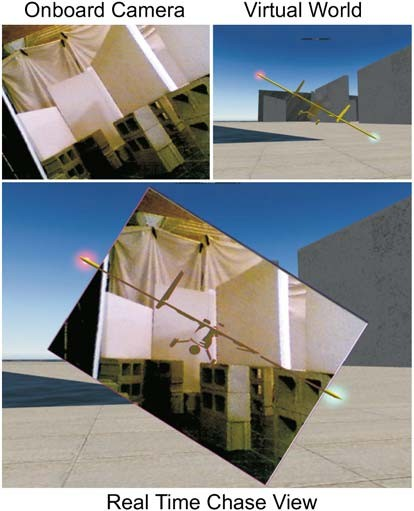
\includegraphics[width=0.48\textwidth]{hing_chase_view}
    \caption[Hing et al. chase view]{Hing et al.'s chase view.\cite{hing2009}}
    \label{fig:hing_chase_view}
  \end{wrapfigure}

  Several methods to show a robotic avatar in a virtual environment were proposed.

  \textcite{nielsen2007} presented an interface in which a \gls{3d} model of the robot, a video stream from a mounted camera, a map, and pose information, were combined in a mixed-reality display.
  \textcite{kelly2011} extended the concept to an outdoor environment, and succeeded in making their system work in various low-throughput situations.
  However, most methods require many sensors, such as \glspl{lrf}, which add expense and weight to the vehicle.

  \textcite{hing2009} succeeded in making a chase view for a fixed-wing \gls{uav}, as shown in \fref{fig:hing_chase_view}.
  This showed the orientation of the drone with respect to the environment, overlaid onto a rotated onboard camera view.
  They were successful in improving flying, and even people who were not able to complete the course using the onboard view alone were able to complete it with the chase view.

\section{Teleoperation System Using Past Image Records}
  \textcite{shiroma2004} introduced a \gls{spir}, a past-image view technique for mobile robots.
  This technology enabled the operator to ascertain the position and orientation of the robot with respect to its environment from a third-person (bird's-eye view) perspective using only camera and pose information.
  A system overview is shown in \fref{fig:spir_system_overview}.

  \begin{figure}[h]
    \centering
    \begin{subfigure}[b]{0.45\textwidth}
      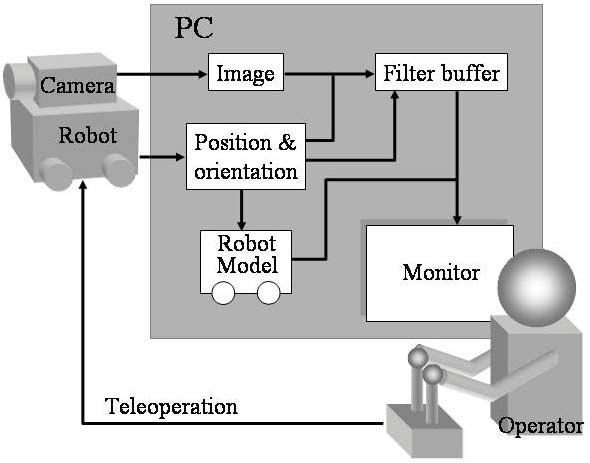
\includegraphics[width=\textwidth]{spir_system_overview}
    \end{subfigure}
    \hfill
    \begin{subfigure}[b]{0.45\textwidth}
      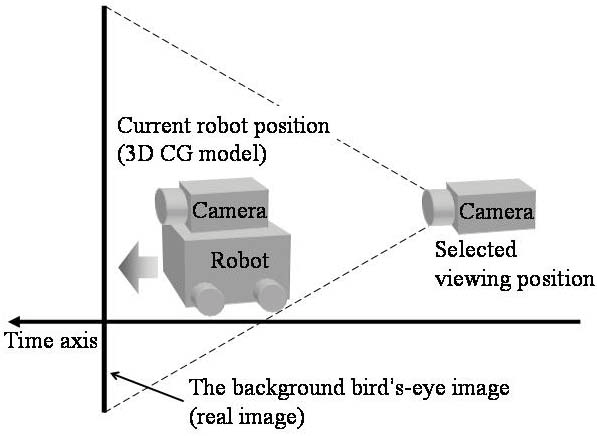
\includegraphics[width=\textwidth]{spir_birdseye}
    \end{subfigure}
    \caption[\acrshort{spir} system overview]{System overview of \gls{spir}.\cite{shiroma2004}}
    \label{fig:spir_system_overview}
  \end{figure}

  Images taken by a raised camera were saved in a buffer along with their position and the time at which they were taken.
  No images are stored while the robot is not moving.
  Three evaluation functions were proposed to select an optimal image to use as the background:

  \begin{description}
    \item [Fixed time delay:] Use images taken a certain period earlier.
    \item [Fixed distance:] Use images taken at approximately the given distance.
    \item [\Gls{fov} evaluation:] Select the closest image if the robot is in the field of view.
  \end{description}

  \fref{fig:spir_naive_algorithms} shows the algorithms for fixed time delay and fixed distance.

  \begin{figure}[h]
    \centering
    \begin{subfigure}[b]{0.45\textwidth}
      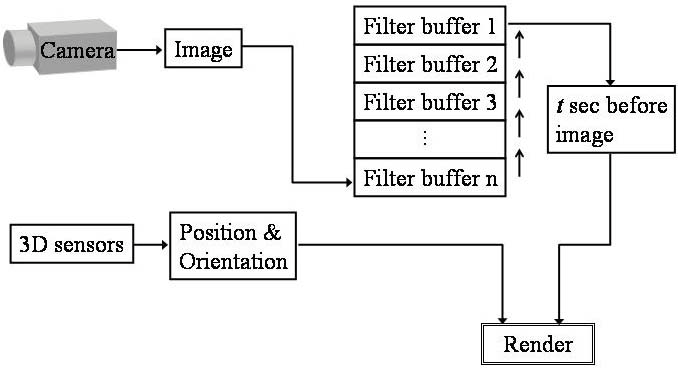
\includegraphics[width=\textwidth]{spir_time_delay}
      \caption{Fixed time delay algorithm.}
      \label{fig:spir_time_delay}
    \end{subfigure}
    \hfill
    \begin{subfigure}[b]{0.45\textwidth}
      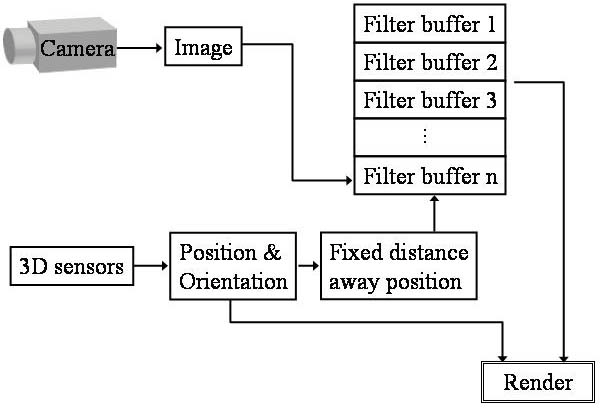
\includegraphics[width=\textwidth]{spir_fixed_distance}
      \caption{Fixed distance algorithm.}
      \label{fig:spir_fixed_distance}
    \end{subfigure}
    \caption[\acrshort{spir} naïve algorithms]{The naïve algorithms.\cite{shiroma2004}}
    \label{fig:spir_naive_algorithms}
  \end{figure}

  \Gls{fov} evaluation uses the fixed-distance algorithm as the base, but also calculates view and centreline distances, as well as the widths at the bottom and centre of the image.
  The definition of the distances, as well as the algorithm, are shown in \fref{fig:spir_fov}.

  \begin{figure}[h]
    \centering
    \begin{subfigure}[b]{0.3\textwidth}
      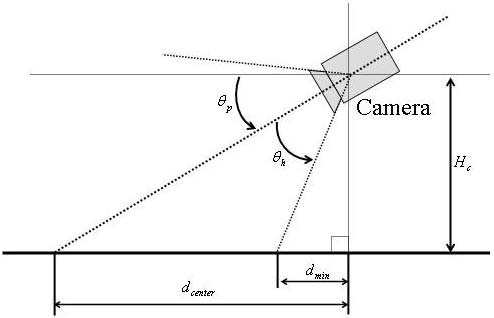
\includegraphics[width=\textwidth]{spir_fov_side_view}
      \caption{Side view.}
      \label{fig:spir_fov_side_view}
    \end{subfigure}
    \hfill
    \begin{subfigure}[b]{0.3\textwidth}
      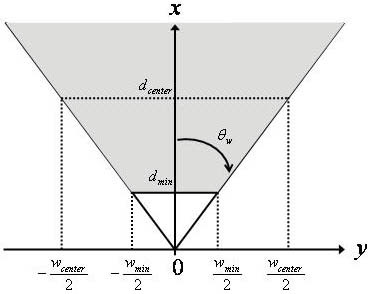
\includegraphics[width=\textwidth]{spir_fov_top_view}
      \caption{Top view.}
      \label{fig:spir_fov_top_view}
    \end{subfigure}
    \hfill
    \begin{subfigure}[b]{0.3\textwidth}
      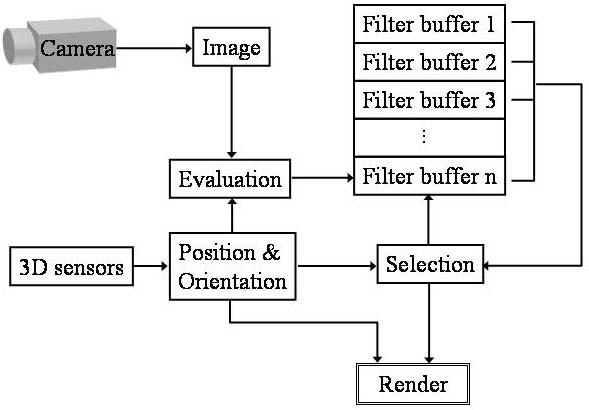
\includegraphics[width=\textwidth]{spir_fov}
      \caption{\Gls{fov} evaluation algorithm.}
      \label{fig:spir_fov_flowchart}
    \end{subfigure}
    \caption[\acrshort{spir} \gls{fov} evaluation algorithm]{\Gls{fov} evaluation.\cite{shiroma2004}}
    \label{fig:spir_fov}
  \end{figure}

  An optimal image was then found using an evaluation function considering several constraints, including \gls{fov} and the relative positions of the camera and robot.
  The latest image is used if no good solution can be found.

  If the bandwidth is low, old images can be reused, updated by an array of position data sent at a higher speed than the video.

  \subsection{Further development}
    \textcite{sugimoto2005} demonstrated the effectiveness of \gls{spir} with user experiments.
    \textcite{ito2008} decreased choppiness by proposing wider \glspl{fov}, and zooming into the background and model as the robot went further into the image plane.
    They also experimented with adding trajectory forecasting to unmanned ground vehicle interfaces.
    Screenshot of \textcite{ito2008} are shown in \fref{fig:zoom_results}.

    \begin{figure}[h]
      \centering
      \begin{subfigure}[b]{0.45\textwidth}
	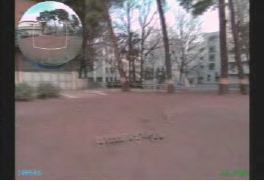
\includegraphics[width=\textwidth]{zoom_live}
      \end{subfigure}
      \hfill
      \begin{subfigure}[b]{0.45\textwidth}
	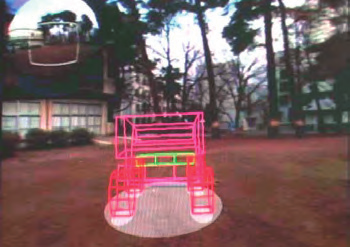
\includegraphics[width=\textwidth]{zoom_combined}
      \end{subfigure}
      \caption[\acrshort{spir} with zoom]{Zoom with bird's-eye view synthesis.\cite{ito2008}}
      \label{fig:zoom_results}
    \end{figure}

    \textcite{murata2014} extended the concept to \gls{3d} when they applied it to mobile manipulators.
    They showed a significant decrease in operators' position error in the vertical direction with a similar error in the longitudinal direction.
    This system is shown in \fref{fig:manip_results}.

    \begin{figure}[h]
      \centering
      \begin{subfigure}[b]{0.45\textwidth}
	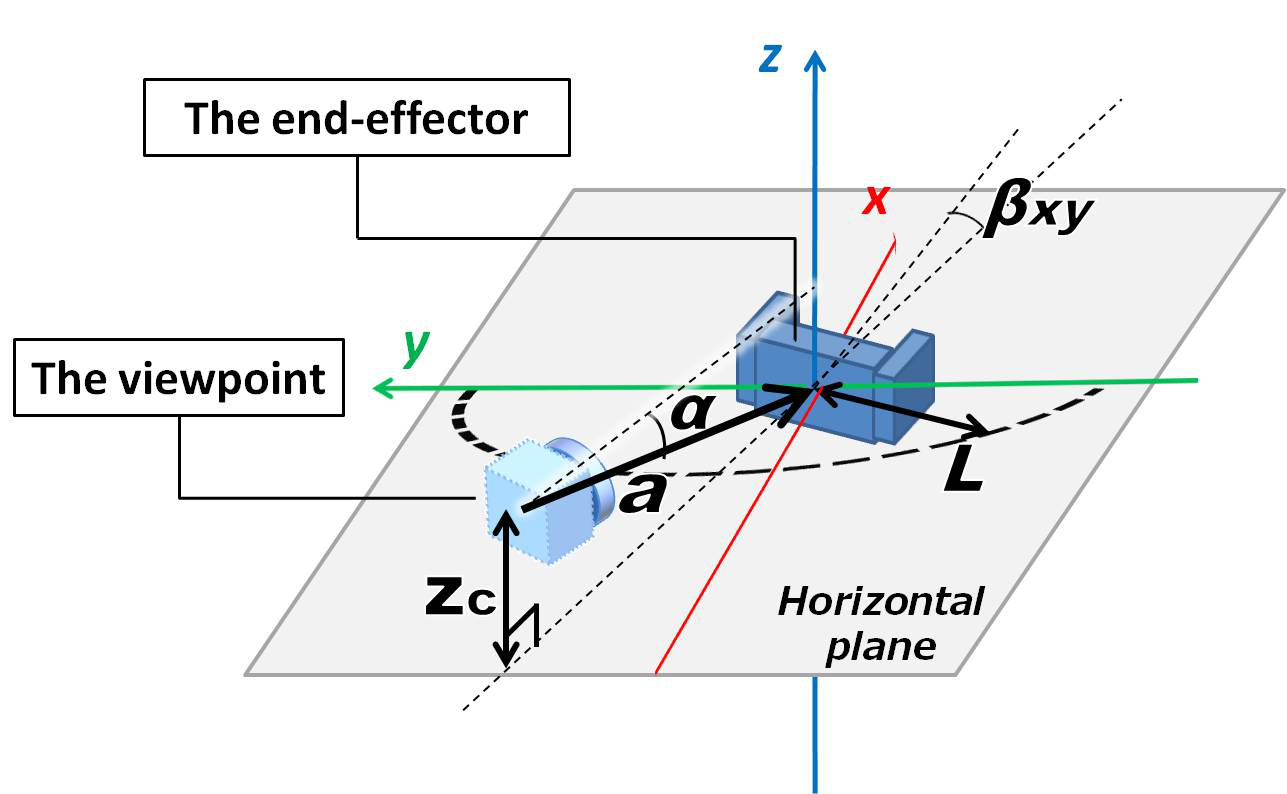
\includegraphics[width=\textwidth]{manip_overview}
	\caption{Geometric relationships.}
	\label{fig:manip_overview_background}
      \end{subfigure}
      \hfill
      \begin{subfigure}[b]{0.45\textwidth}
	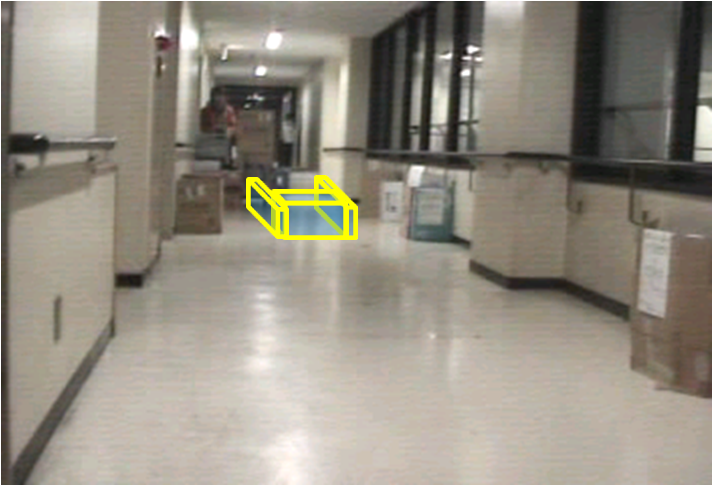
\includegraphics[width=\textwidth]{manip_result}
	\caption{Basic display concept.}
      \end{subfigure}
      \caption[\acrshort{spir} with mobile manipulator]{\gls{spir} used with a mobile manipulator.\cite{murata2014}}
      \label{fig:manip_results}
    \end{figure}

\section{Problems of applying SPIR to quadrotors}
  When a quadrotor flies forwards, the craft pitches down.
  For cameras which do not offer gimballing or a wide \gls{fov}, though, this means that the horizon could go out of frame.
  As a result, older video would need to be used, which would likely be from a longer distance.
  If the drone turns while going forward, the only usable images might be the live ones.

  One potential mitigating factor would be to set a maximum pitch angle, though that would limit the speed of the drone.
  Even so, during straight and level flight, an operator would only be able to see the drone from behind, unless an elevated camera is attached.

  Another possible solution would be to tilt the camera upwards.
  This would limit the amount of ground it would see during a hover.
  In addition, it would cause the camera to be pointing at the sky while the drone is outdoors and moving backwards, removing potential reference points.

  Finally, localization can be difficult too.
  Even outdoors, \gls{gps} only tends to be accurate to within a few metres, which is much larger than the widths of most drones.
  While estimates of acceleration can be obtained by modelling the motor outputs and using built-in accelerometers and gyroscopes, there is often drift from wind, as well as significant vibration even during hovering.
  Integrating acceleration twice to obtain position would cause exponentially increasing drift.

  External sources could be used to reduce the error, such as motion capture cameras if indoors, binocular cameras, visual odometry, \gls{gps}, or \gls{slam}.
  That might require the use of more additional tools, such as ultrasonic distance sensors or laser range finders.
  An \gls{ekf} could then be used to estimate the best location and minimize drift.
  However, that is beyond the scope of this research.

  Some \gls{slam} algorithms, such as \gls{ptam}, \gls{rtslam}, or \gls{lsdslam}, are able to use monocular cameras, but rotation on the spot often causes them to lose keypoints, making them a bad choice for drones.

% TODO:
% ・結局、本研究では何をやるのか?
% ・なぜ、それをやる必要があるのか?
% ・何が新しいのか?
% ・それをやるには、何が困難なのか?
% ・そして、それをどのようにクリアしたのか?
% 
% これらをまとめること。
